%%%%%%%%%%%%%%%%%%%%%%%%%%%%%%%%%%%%%%%%%%%%%%%%%%%%%%%%%%%%%
\section{Header}\label{header}
%%%%%%%%%%%%%%%%%%%%%%%%%%%%%%%%%%%%%%%%%%%%%%%%%%%%%%%%%%%%%

%%%%%%%%%%%%%%%%%%%%%%%%%%%%%%%%%%%%%%%%%%%%%%%%%%%%%%%%%%%%%
\subsection{Preamble}\label{header:preamble}
%%%%%%%%%%%%%%%%%%%%%%%%%%%%%%%%%%%%%%%%%%%%%%%%%%%%%%%%%%%%%

The file starts with a header, with the following structure:

\begin{verbatim}
struct Header {
  byte        magic_number[8];
  le_uint32   version;
  le_uint32   header_len;
  byte        header_data[header_len];
};
\end{verbatim}

The \kw{magic\_number} is the ASCII representation of the string ``crypt4gh''.

The version number is stored as a four-byte little-endian unsigned integer.
%
The current version number is 1.

\kw{header\_len} is the length of the \emph{remainder} of the header, stored as a four-byte little-endian unsigned integer.


The current byte representation of the magic number and version is:
\begin{verbatim}
0x63 0x72 0x79 0x70 0x74 0x34 0x67 0x68 0x01 0x00 0x00 0x00
============= magic_number============= ===== version =====
\end{verbatim}


%%%%%%%%%%%%%%%%%%%%%%%%%%%%%%%%%%%%%%%%%%%%%%%%%%%%%%%%%%%%%
\subsection{Header Data}\label{header:data}
%%%%%%%%%%%%%%%%%%%%%%%%%%%%%%%%%%%%%%%%%%%%%%%%%%%%%%%%%%%%%

This section describes how the parameters, used to encrypt the application data, are themselves serialized %stored
and encrypted.
%
The \kw{header\_data} sequence of bytes is organized using the type \kw{HeaderData}, as follows:

\begin{verbatim}
enum EncryptionMethod<le_uint32> {
  chacha20_ietf_poly1305 = 0;
};

struct HeaderData {
  enum EncryptionMethod<le_uint32> header_encryption_method;
  select (header_encryption_method) {
    case chacha20_ietf_poly1305:
      byte                         public_key[32];
      byte                         nonce[12];
  };
  byte[]                           encrypted_header;
};
\end{verbatim}

\begin{figure}
 \centering
 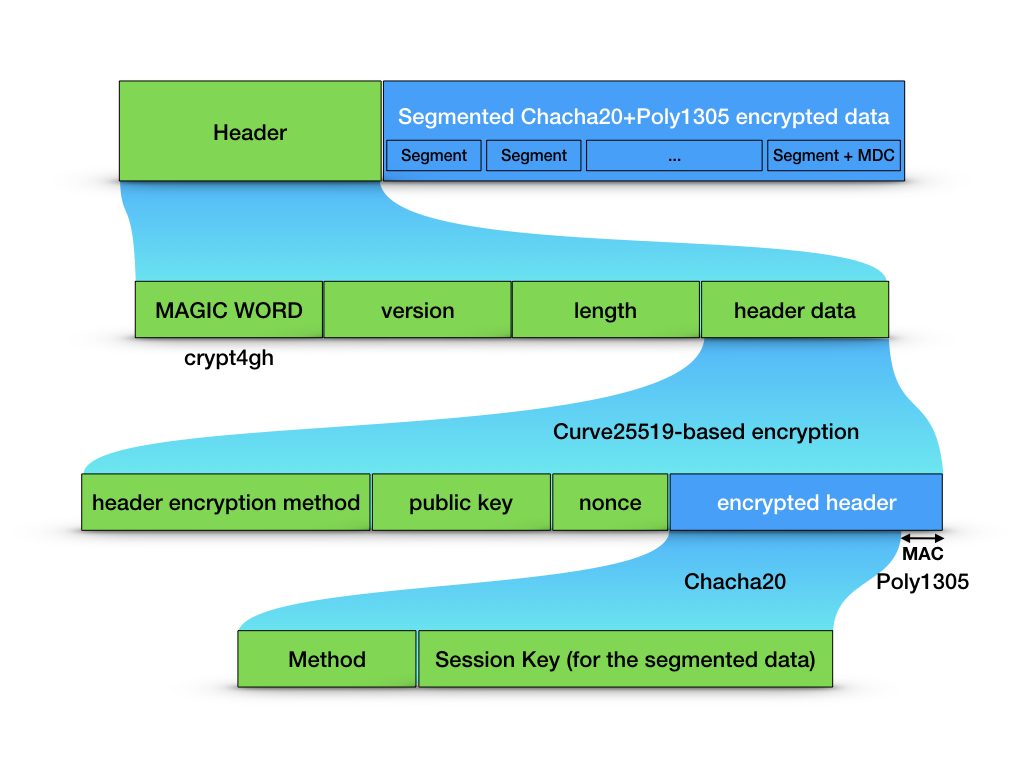
\includegraphics[width=\textwidth]{sections/encryption.png}
 \caption{Structure of the Header}
 \label{figure:header:structure}
\end{figure}


\kw{header\_encryption\_method} is an enumerated type that describes how the \kw{encrypted\_header} is generated.

The plaintext of the \kw{encrypted\_header} encodes, using the following type \kw{EncryptionParameters}, the parameters used for the encryption of the data portion.
%
The plaintext is then encrypted as stipulated by the \kw{header\_encryption\_method} (See Section~\ref{header:encrypted}).

\begin{verbatim}
enum EncryptionMethod<le_uint32> {
  chacha20_ietf_poly1305 = 0;
};

enum ChecksumAlgorithm<le_uint32> {
  none = 0;
  md5 = 1;
  sha256 = 2;
};

struct EncryptionParameters {
  enum ChecksumAlgorithm<le_uint32> checksum_algorithm;

  enum EncryptionMethod<le_uint32>  method;
  select (method) {
    case chacha20_ietf_poly1305:
      byte                          key[32];
  };
};
\end{verbatim}

% ---------------
\kw{method} is an enumerated type that describes the type of encryption to be used.

\kw{key} is a secret encryption key.
%
In the case of \kw{chacha20\_ietf\_poly1305}, it is a sequence of 32 bytes.

% ---------------
\kw{checksum\_algorithm} is an enumerated type that describes how the checksum over the \emph{unencryted} data content is computed.
%
If a checksum algorithm is chosen, `sha256' SHOULD be prefered and `md5' SHOULD only be used for backwards compatibility.
%
Moreover, the checksum value is of the following form and appended at the end of the encrypted data portion (see Section~\ref{data:encrypted}). Nothing is appended if \kw{checksum\_algorithm} is \kw{none}.
%
\begin{verbatim}
select (checksum_algorithm) {
  case md5:
    byte       key[16];
  case sha256:
    byte       key[32];
  };
\end{verbatim}

% The following is an example of a header configuration:
% %
% \begin{verbatim}
% [magic number][version][header len][header enc. method][pubkey][nonce][enc. header][mac]
% \end{verbatim}


%%%%%%%%%%%%%%%%%%%%%%%%%%%%%%%%%%%%%%%%%%%%%%%%%%%%%%%%%%%%%
\subsection{Encrypted Header}\label{header:encrypted}
%%%%%%%%%%%%%%%%%%%%%%%%%%%%%%%%%%%%%%%%%%%%%%%%%%%%%%%%%%%%%

The header data is encrypted using a Curve25519-based asymmetric encryption.
%
Informally, Curve25519-based asymmetric encryption uses the Currve25519 ECC function to generate a shared encryption key from the encrypter's private key and the recipient's public key, which can be re-created by the recipient using its secret key and the encrypter's public key.
%

% ---------------------------------
The \kw{encrypted\_header} is generated by encrypting the header data, following the \kw{header\_encryption\_method}.
%
In the case of \kw{chacha20\_ietf\_poly1305}, it is encrypted using ChaCha20 and authenticated using Poly1305~\cite{RFC8439}, using the same algorithms described in Section~\ref{data:encrypted:chacha20poly1305}.
%
The public key of the encrypter and the randomly-generated nonce, used in the encryption, are prepended, and the Poly1305 authentication tag is appended.


The shared key, used by Chacha20, is calculated using X25519 ECC function as it is described in~\cite{RFC7748} (section 5).
%

The public key can be used as proof of origin of the encrypted file.
%
